\documentclass{article}
\usepackage{caption} % Caption mynda
\usepackage{hyperref}
\usepackage{graphicx, float} % Insetning mynda
\usepackage{keystroke} % Veit ekki
\usepackage{pgfplots} % Veit ekki
\usepackage{enumerate} % Numbered-bullet-points
\usepackage{amsmath} % E.g. for formatting equations without numbers (equation*)
\usepackage{listings} % Insert code to document
\pgfplotsset{compat=1.17}
% \usepackage{showlabels}
\usepackage[T1]{fontenc} % Encoding
\usepackage[utf8]{inputenc} % Encoding
% \usepackage[icelandic]{babel} %Encoding

\usepackage{geometry}
\geometry{
    paper=a4paper, % letterpaper lika til
	top=2.5cm, % Top margin
	bottom=2cm, % Bottom margin
	left=3.5cm, % Left margin
	right=3.4cm, % Right margin
	headheight=0.75cm, % Header height
	footskip=1cm, % Space from the bottom margin to the baseline of the footer
	headsep=0.75cm, % Space from the top margin to the baseline of the header
	%showframe, % Uncomment to show how the type block is set on the page
}
    
% \usepgfplotslibrary{units}
\RequirePackage{fancyhdr}
\linespread{1.3} % Línubil
\fontfamily{pbch}\selectfont
\usepackage{color}

\definecolor{mygreen}{rgb}{0,0.6,0}
\definecolor{mygray}{rgb}{0.5,0.5,0.5}
\definecolor{mymauve}{rgb}{0.58,0,0.82}
\lstset{
showstringspaces=false,
backgroundcolor=\color{white},
basicstyle=\footnotesize,
breaklines=true,
captionpos=b,
commentstyle=\color{mygreen},
keywordstyle=\color{blue},
stringstyle=\color{mymauve},
}

% \usepackage{zref}
% \usepackage{biblatex} %Imports biblatex package
%\usepackage[backend=biber]{biblatex}
%\addbibresource{references.bib} %Import the bibliography file
\begin{document}

\today \par
\vspace{.5cm}
\noindent Háskólinn í Reykjavík, Embedded Systems Programming, \textbf{Project 1} \par
\noindent \textbf{Eyþór Mikael Eyþórsson}, \texttt{eythore19@ru.is}\par
\noindent \textbf{Ólafur Þórsson}, \texttt{olafurth24@ru.is}\par
\noindent \textbf{Vilhjálmur Páll Thorarensen}, \texttt{vilhjalmurt19@ru.is}\par
%\noindent Instructors: \textbf{TEACHER} \par

\section*{About the assignment}
The code was implemented in a manner such that it executes parts of the assignment based
on compiler arguments, i.e. uncommenting the \texttt{// \#define PART1} line in
\texttt{main.cpp} makes the code execute part 1. The same goes for part 2 and 3 with the
complication that part 1 and 3 have conditional code in \texttt{encoder\_driver.cpp}.

The oscilloscope was set up the same during the whole project, i.e. one pole connected to
ground and the other to C1.
The video can be found \href{https://youtu.be/15Uzd80X8S8}{here} and the codebase
\href{https://github.com/mikaeleythor/embe-project-1}{here}.


\section*{Part 1}
To keep things convenient for engineering students, pulse rate was defined as the number
of positive edges per second, which has the unit $Hz$.
\subsection*{Max pulse rate}
The maximum pulse rate of the motor was found using the following formula: \[
	\text{max pulse rate} = \frac{\text{motor speed in rpm} \cdot \text{max pulses per
			revolution}}{60s}
\] which yielded \[
	\text{max pulse rate} = \frac{155rpm \cdot (7\cdot 100)ppr}{60s} \approx 1808Hz
\] for the no-load motor speed. The oscillosscope measured 1776Hz while the motor was
powered by a programmable DC power supply at 6V.

\subsection*{Max time between samples}
The minimum sample rate was found using the Shannon Sampling Theorem, which
states that the sample rate must be at least twice the bandwidth of the signal to avoid
aliasing. Consequently, the maximum time between samples can be determined via \[
	\text{max time between samples} = \frac{1}{2*\text{pulse rate}} =
	\frac{1}{2\cdot1808Hz} = 276\mu s
\]

\subsection*{Max response time}
To detect direction, a second encoder signal which is shifted by 90\textdegree{} is added
and so, to correctly determine the direction, the response time must be at maximum half of
the max time between samples, i.e. $\frac{276\mu s}{2} = 138\mu s$. The corresponding
sampling rate can be calculated as \[
	\text{sampling rate} = \frac{1}{138\mu s}Hz = 7246Hz
\]

The response time was tested on the oscilloscope by adding delays to the input signal,
on each side of the threshold, yielding that delays under $180\mu s$ yielded a stable
light from an LED which turns on when the motor rotates clockwise, while delays over
$190\mu s$ yielded no light from the LED.


\subsection*{Counting}
The counting was performed using the oscilloscope. Experiments were performed in a manner
such that pulses were counted during an approximately 10s interval, then a computed count
was transmitted through UART. A single twist of the motor yielded a count on the
oscilloscope (Figure \ref{fig:osc}) which was approximately half of the pulses transmitted via UART.

\begin{figure}[h]
	\begin{center}
		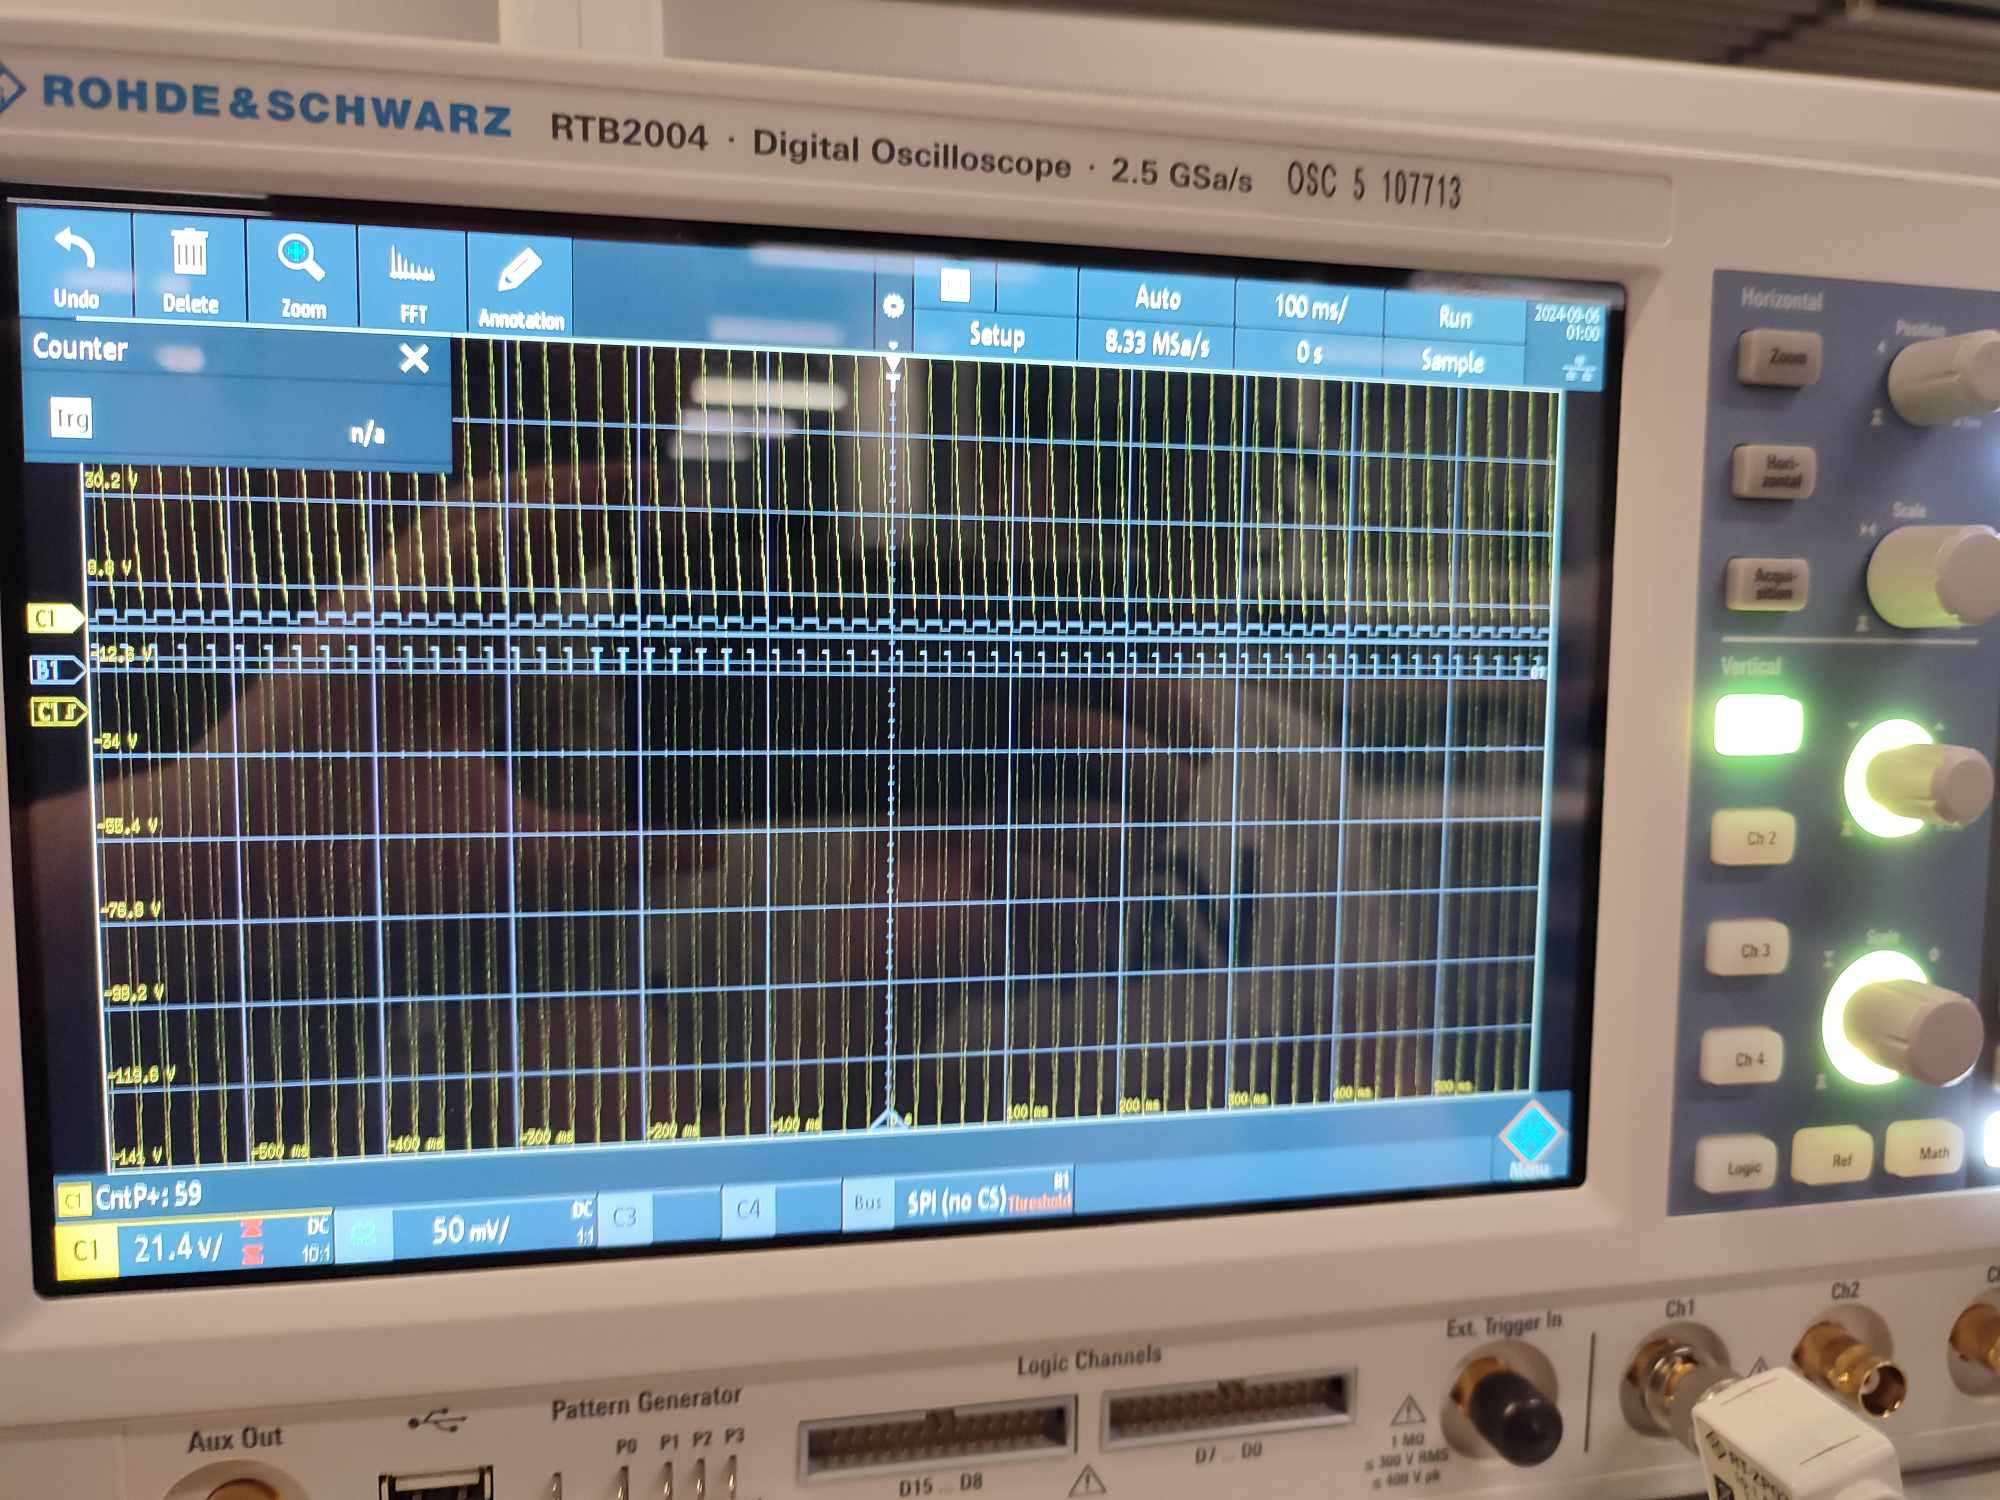
\includegraphics[width=0.95\textwidth]{./oscilloscope.jpeg}
	\end{center}
	\caption{59 pulses were counted in 10s after a single twist of the motor. This roughly
		matched the 120 edges that were counted by the microcontroller}\label{fig:osc}
\end{figure}

\section*{Part 2}
Printing inside the main loop in each iteration resulted in the counter to miss pulses.
The oscilloscope showed 113 pulses and the UART countar was 52 (a correct output would be
56).

\section*{Part 3}
The C1 pin was connected in parallel to both PB1 and PD2. PD2 was used to trigger the
interrupt (which was implemented inside the Encoder), and PB1 was used to read the value
in the same manner as before. The results were an increased accuracy in the UART output
and a stronger correlation between the oscilloscope and the UART. The UART was also more
comfortable to work with and more stable, i.e. spacing the print statements between 3s of
down time made the output more readable.

%\newpage
%\printbibliography

\end{document}
